
\chapter{Analysis}
In this chapter, the data generated from the experiments presented in the previous chapter are analyzed. The preprocessing methods used on the data is discussed, the metrics used in evaluating the correspondence between image detections and lidar data are introduced, and the results from each experiment are presented.
\section{Preprocessing}
In order to associate boat detections in the images to world coordinates, the inverse calibration matrix from equation \ref{eq:calibr} using the values found for the matrix $\mathcal{K}$ in section \ref{section:matlab_calibration} was multiplied with the pixel coordinates of the center point of the bounding boxes found by the faster R-CNN implementation. This associates the pixel coordinates with the normalized image plane presented in figure \ref{fig:image_coordinates} in section \ref{section:camera_coordinates}, giving a direction to the center of the bounding box valid up to a scale factor. Due to the image data being in 2D coordinates, one is only able to associate a detection in an image with a direction, or ray, in 3D space. This ray was subsequently transformed from the camera frame, denoted $c$, to the lidar frame of reference, denoted $l$, using the rotation matrix
\begin{equation}
\mathcal{R}_c^l=\begin{bmatrix}
\cos{\frac{\pi}{2}} & -\sin{\frac{\pi}{2}} & 0 \\
\sin{\frac{\pi}{2}} & \cos{\frac{\pi}{2}} & 0 \\
0 & 0 & 1
\end{bmatrix}\begin{bmatrix}
\cos{-\frac{\pi}{2}} & 0 & \sin{-\frac{\pi}{2}}\\
0 & 1 & 0 \\
-\sin{-\frac{\pi}{2}} & 0 & \cos{-\frac{\pi}{2}}
\end{bmatrix}=\begin{bmatrix}
0 & 0 & 1\\
-1 & 0 & 0\\
0 & -1 & 0
\end{bmatrix}
\end{equation}
which is a rotation of $\frac{\pi}{2}$ radians around the cameras z-axis, followed by a rotation of $-\frac{\pi}{2}$ radians around the new y-axis, and the translation vector
\begin{equation}
\mathbf{t_c^l}=\begin{bmatrix}
-0.05 & 0 & -0.097
\end{bmatrix}^T
\end{equation} 
given in meters. The rotation angles and translation vector were measured by hand.

The location used in the experiments gave many returns in the lidar point cloud from the surroundings, which can be considered clutter or noise in the measurements when the task is locating the boat. Figure \ref{fig:ravnkloa_pointcloud} shows a point cloud of the surroundings projected down to two dimensions, illustrating the many unwanted returns. The red circle indicates the area where the maneuvers were performed, and the black arrow indicate the flow of the Nidelven river. 
\begin{figure}[H]
	\centering
	\includegraphics[width=\linewidth]{fig/ravnkloa_surroundings.png}
	\caption{The lidar point cloud including surroundings at Ravnkloa, projected down to the xy-plane.}
	\label{fig:ravnkloa_pointcloud}
\end{figure}
Since, unfortunately, no position ground truth was produced during the experiments, it was decided to use the returns from the boat in the lidar data as a ground truth, when comparing detections from faster R-CNN with the lidar data. In order to achieve this, all unwanted returns were filtered using a "pass through" filter removing all points which lies outside a specified rectangular region in the xy-plane, keeping only the returns from the boat. The point cloud was also reduced to two dimensions by projecting all points down to the plane $z=0$, for simplicity \todo{mer}.

Once the point cloud was reduced to two dimensions, and all returns not belonging to the target boat was removed, k-Means clustering (with k=1) was used to find the centroid of the points returned by the boat.
\section{Metrics}
Faster R-CNN gives the bounding boxes for its detections, along with the score for the detection, indicating the "confidence" in the classification. The threshold for the score was set to 0.6, where 1.0 indicates absolute certainty (from the detectors perspective) and 0 indicates zero confidence. The 0.6 threshold was the default set in the faster R-CNN implementation from the Github repository. The detection threshold has not been analyzed with particular attention in this project, due to limited time, so the default threshold has been kept as-is.

As a metric in determining whether or not a detection from the convolutional net corresponds with the boat, the minimum distance between the ray projected by the centroid of the bounding box and the centroid of the point cloud cluster corresponding to the boat was used. This distance was set to 2.5 meters. This value was heuristically determined through experimentation, and was chosen as a compromise between the target boat being detected versus boats in the background counting as a detection of the target boat. Due to the geometry of the boat, for some maneuvers the majority of the returns found by the lidar come from the front part of the boat, while the detections in the image are more centered on the projection of the boat into the image plane. The 2.5 meters distance also allow for some time delay between the images and the point cloud. The images corresponding to a particular point cloud were found by searching through the image set and selecting the image with the temporally closest time stamp, since the time delay between the lidar and the camera is unknown (but present). Lastly, the transformation between the camera frame and the lidar frame is hand-measured and assumes that the camera z-axis is perfectly aligned with the lidar x-axis, not taking into account misalignments. The minimum distance of 2.5 meters allows for some leeway in the alignment of the sensors.

Consider figure \ref{fig:example_ex3_pc}, and the corresponding image with bounding boxes in figure \ref{fig:example_ex3_im}. The blue dot in figure \ref{fig:example_ex3_pc} is the centroid of the point cloud. Although the bounding box in figure \ref{fig:example_ex3_im} is almost perfectly centered on the target boat, there is a small discrepancy between the point cloud centroid and the projected ray in figure \ref{fig:example_ex3_pc}. This discrepancy is likely due to a combination of time delay between the sensors, the geometry of the point cloud not capturing the full geometry of the boat, as well as misalignment between the sensors. \todo{flytt til diskusjon}.
\begin{figure}[H]
	\centering
	\includegraphics[width=\linewidth]{fig/example_1_pc.png}
	\caption{A single point cloud from experiment 3, with the ray corresponding to the center of the bounding box detected in the image projected out in the scene.}
	\label{fig:example_ex3_pc}
\end{figure}
\begin{figure}[H]
	\centering
	\includegraphics[width=\linewidth]{fig/example_1.png}
	\caption{Image with bounding boxes and scores corresponding to the point cloud in figure \ref{fig:example_ex3_pc}.}
	\label{fig:example_ex3_im}
\end{figure}
Another thing to notice in figure \ref{fig:example_ex3_im} is the fact that there are other boats in the surrounding scene, giving detections other than the target ship. Not only can this give false detections, but it can also lead to a missed detection due to the foreground and background ships being detected as one. Figure \ref{fig:issues_multiple_detections} illustrates two examples where multiple ships are detected as one. \todo{flytt til diskusjon}
\begin{figure}
	\centering
	\begin{subfigure}[t]{.5\textwidth}
		\centering
		\includegraphics[width=\linewidth]{fig/issue_overlapping.png}
		\caption{Three ships detected as one (far left of the image).}
		\label{fig:sub_issue1}
	\end{subfigure}%
	\begin{subfigure}[t]{.5\textwidth}
		\centering
		\includegraphics[width=\linewidth]{fig/issue_2.png}
		\caption{Two ships detected as one (second bounding box from the left).}
		\label{fig:sub_issue2}
	\end{subfigure}
	\caption{Two examples of multiple ships being detected and classified as one.}
	\label{fig:issues_multiple_detections}
\end{figure} 
Given more time, this issue could have been compensated for by for example background subtraction. However, in a realistic situation there is no way of knowing what is the background and what is not, and the problem of target association is an important part of sensor fusion and tracking \todo{fiks}. In order to avoid multiple detections in cases where the target boat pass in front of a boat in the background, only the detection closest to the point cloud cluster center is considered. For each measurement, the number of total image detections are calculated, and an estimate of the probability of detection based on range from the sensors are computed based on the number of image detections versus the number of point clouds in total at that range. The distance between the center of the bounding box and the cluster center is plotted against the distance from the sensors to the center of the point cloud.
\section{Experimental Results}
\subsection{Experiment 1}
Experiment 1 was performed by the vessel arriving head on towards the sensor setup, see figure \ref{fig:experiments}.
The first return from the boat was attained at a range of 67.39 meters, shown in figure \ref{fig:ex1_1}.
\begin{figure}[htbp]
	\centering
	\begin{subfigure}[t]{.5\textwidth}
		\centering
		\includegraphics[width=\linewidth]{fig/detection_1_exp_1.png}
		\caption{First return from the lidar.}
		\label{fig:sub_e1l1}
	\end{subfigure}%
	\begin{subfigure}[t]{.5\textwidth}
		\centering
		\includegraphics[width=\linewidth]{fig/detection_1_exp_1_img.png}
		\caption{Corresponding image from the camera, with bounding boxes overlaid. The target is the smallest rectangle in the center of the image.}
		\label{fig:sub_e1i1}
	\end{subfigure}
	\caption{The first return from the lidar, along with the corresponding detections in the image.}
	\label{fig:ex1_1}
\end{figure}
\begin{figure}[htbp]
	\centering
	\begin{subfigure}[t]{.5\textwidth}
		\centering
		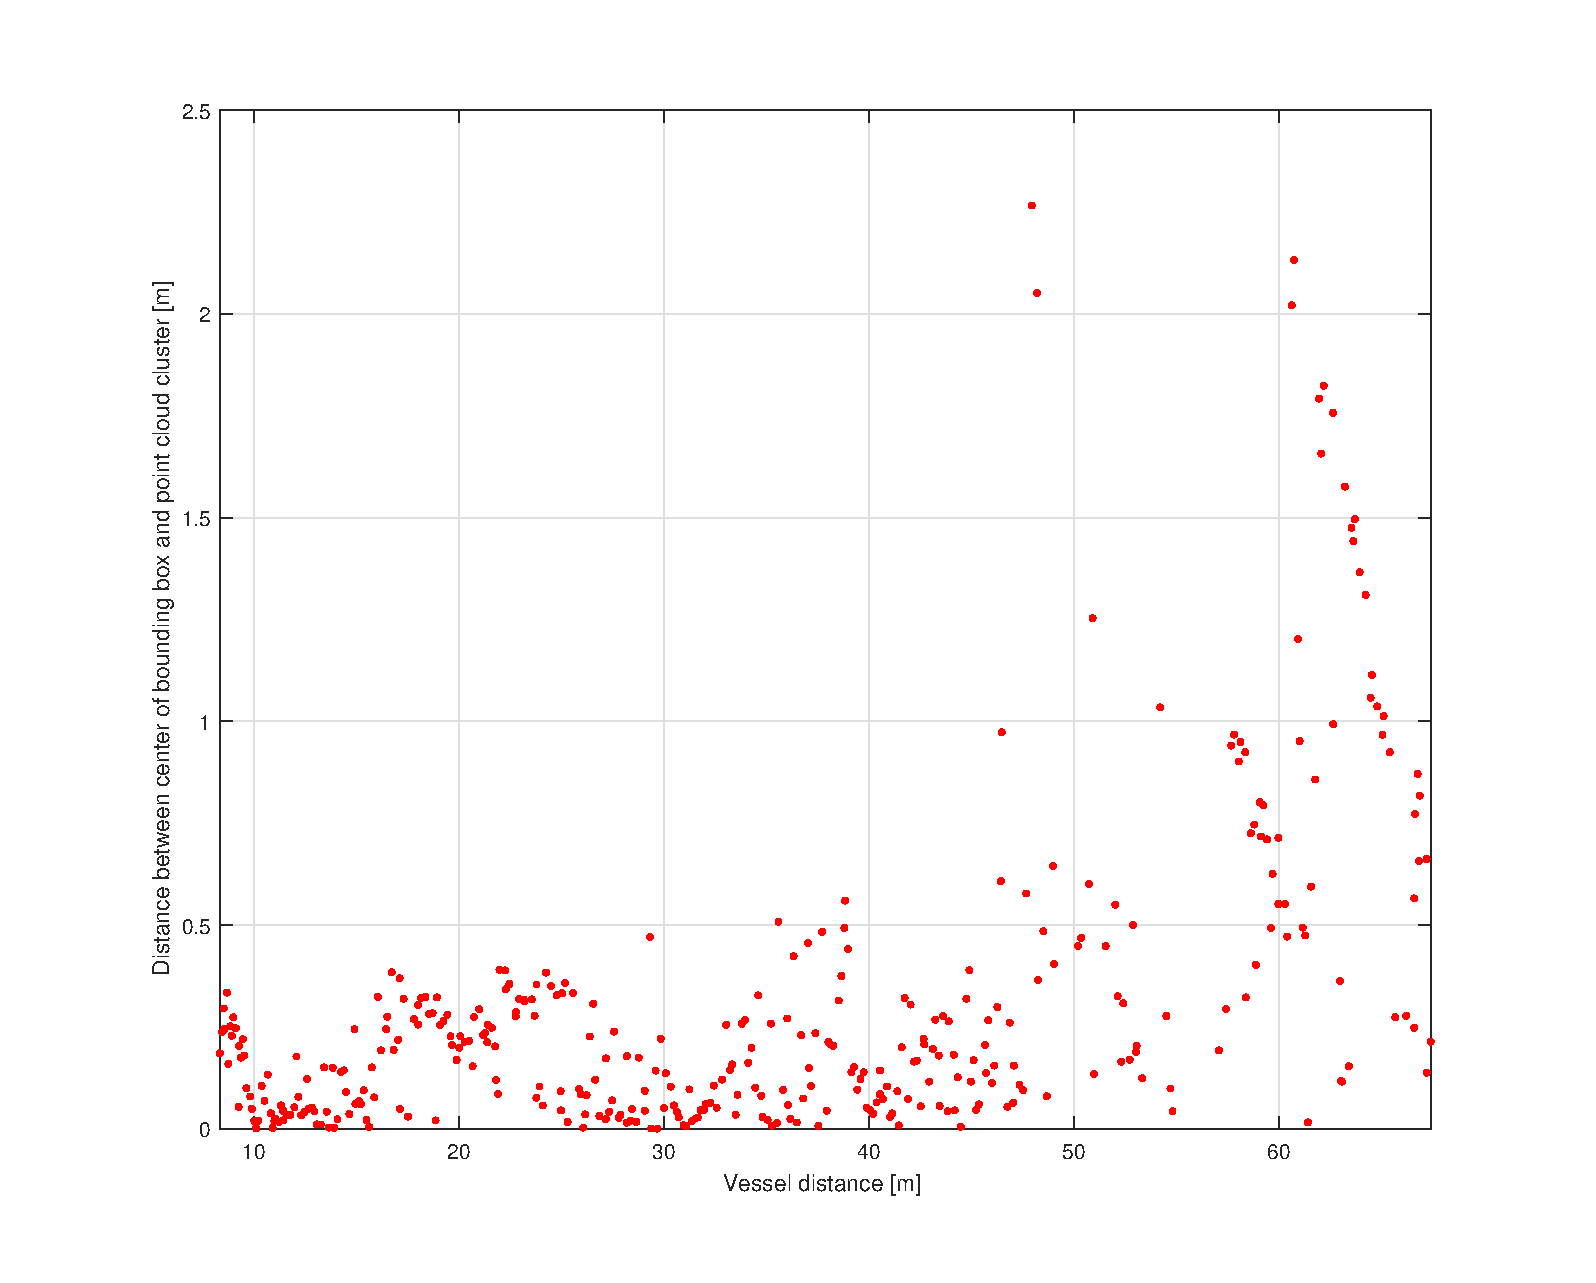
\includegraphics[width=\linewidth]{fig/exp_1_detect_dist.eps}
		\caption{Distance from the center of the bounding\\ box to the point cloud cluster centroid vs.\\ distance to target.}
		\label{fig:sub_ex1_detect_dist}
	\end{subfigure}%
	\begin{subfigure}[t]{.5\textwidth}
		\centering
		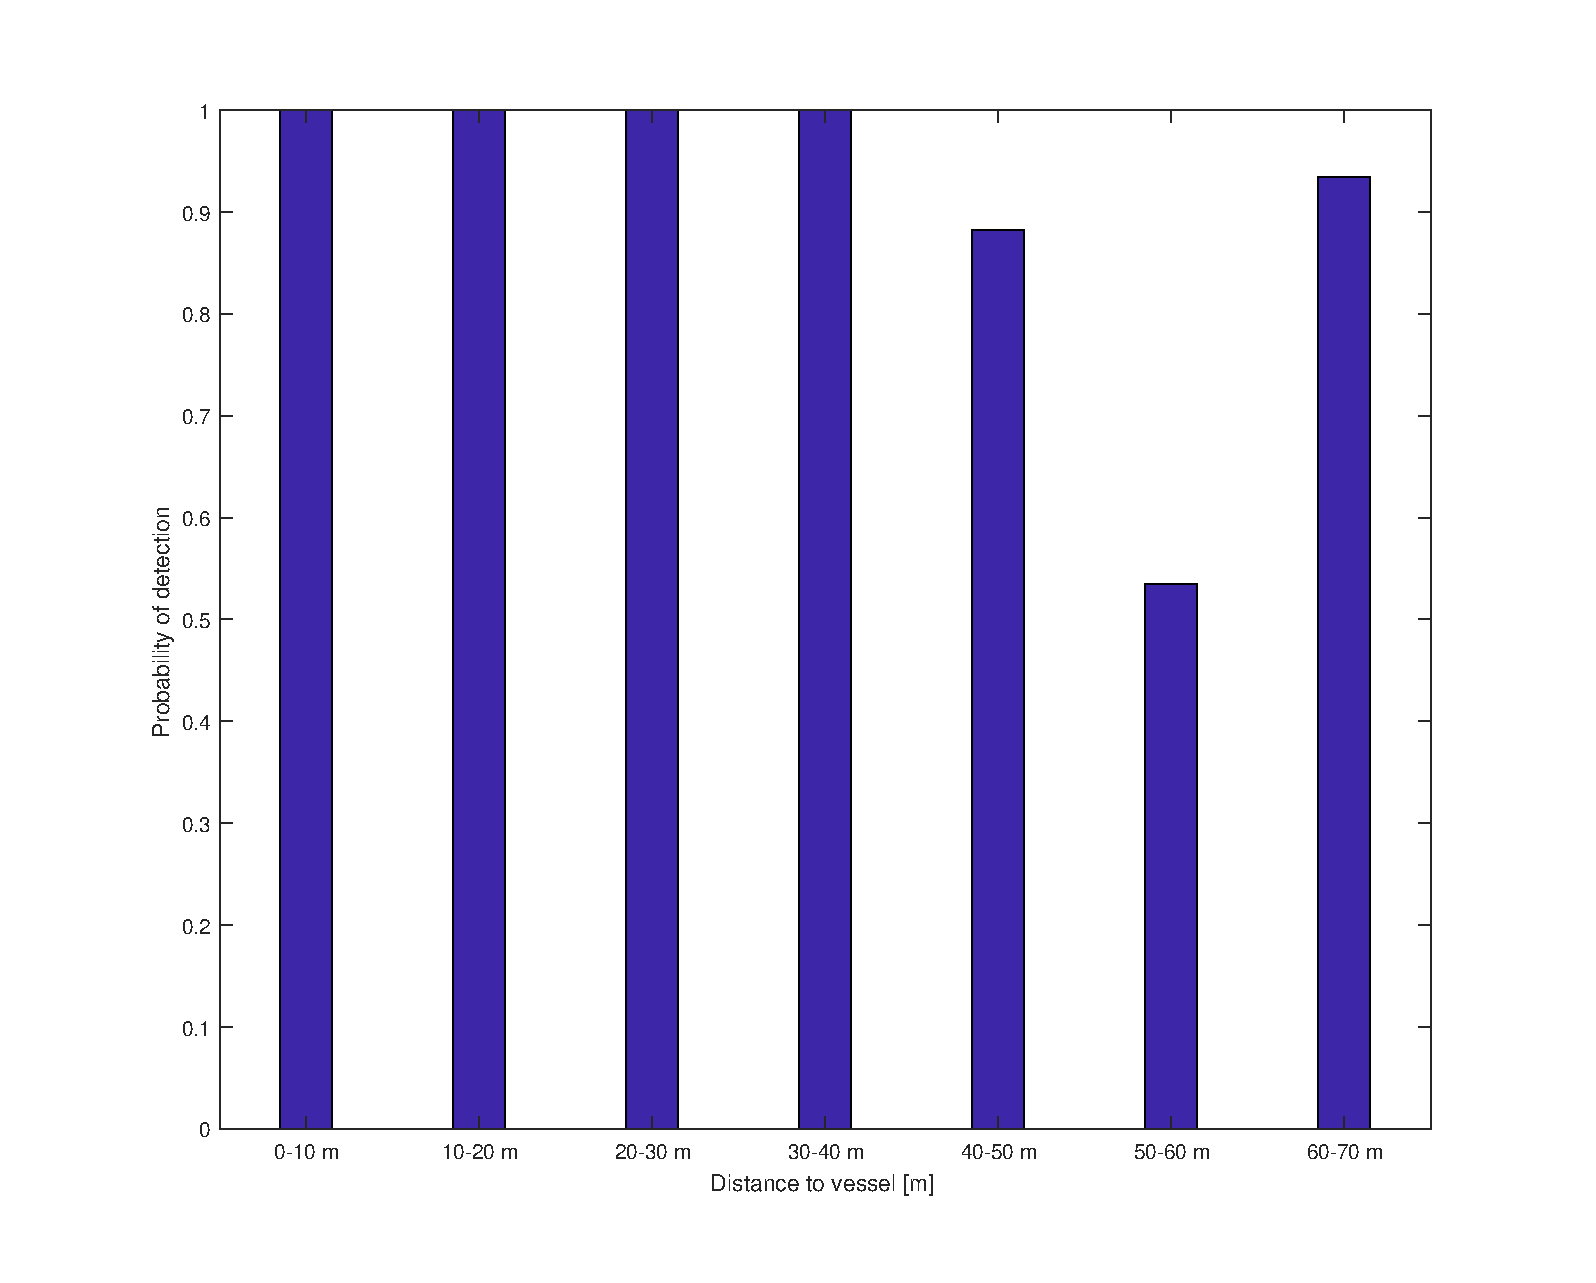
\includegraphics[width=\linewidth]{fig/exp_1_probs.eps}
		\caption{Estimate for probability of detection based on range.}
		\label{fig:sub_ex1_prob}
	\end{subfigure}
	\caption{Results from experiment 1.}
	\label{fig:ex1_plot}
\end{figure}
As figure \ref{fig:ex1_plot} shows, once the vessel was within 40 meters, every single point cloud had a corresponding detection of the vessel.
The total number of point clouds, total number of detections and an estimate of total detection probability is shown in table
\begin{table}[H]
	\centering
	\begin{tabularx}{.7\linewidth}{L c}
		\toprule
		Number of point clouds & 409\\
		\midrule
		Number of detections & 365\\
		\midrule
		Estimated probability of detection in image & 0.8924 \\
		\bottomrule
	\end{tabularx}
\caption{Data from experiment 1.}
\label{tab:exp1}
\end{table}
\subsection{Experiment 2}

\begin{figure}[H]
\centering
\begin{subfigure}[t]{.5\textwidth}
	\centering
	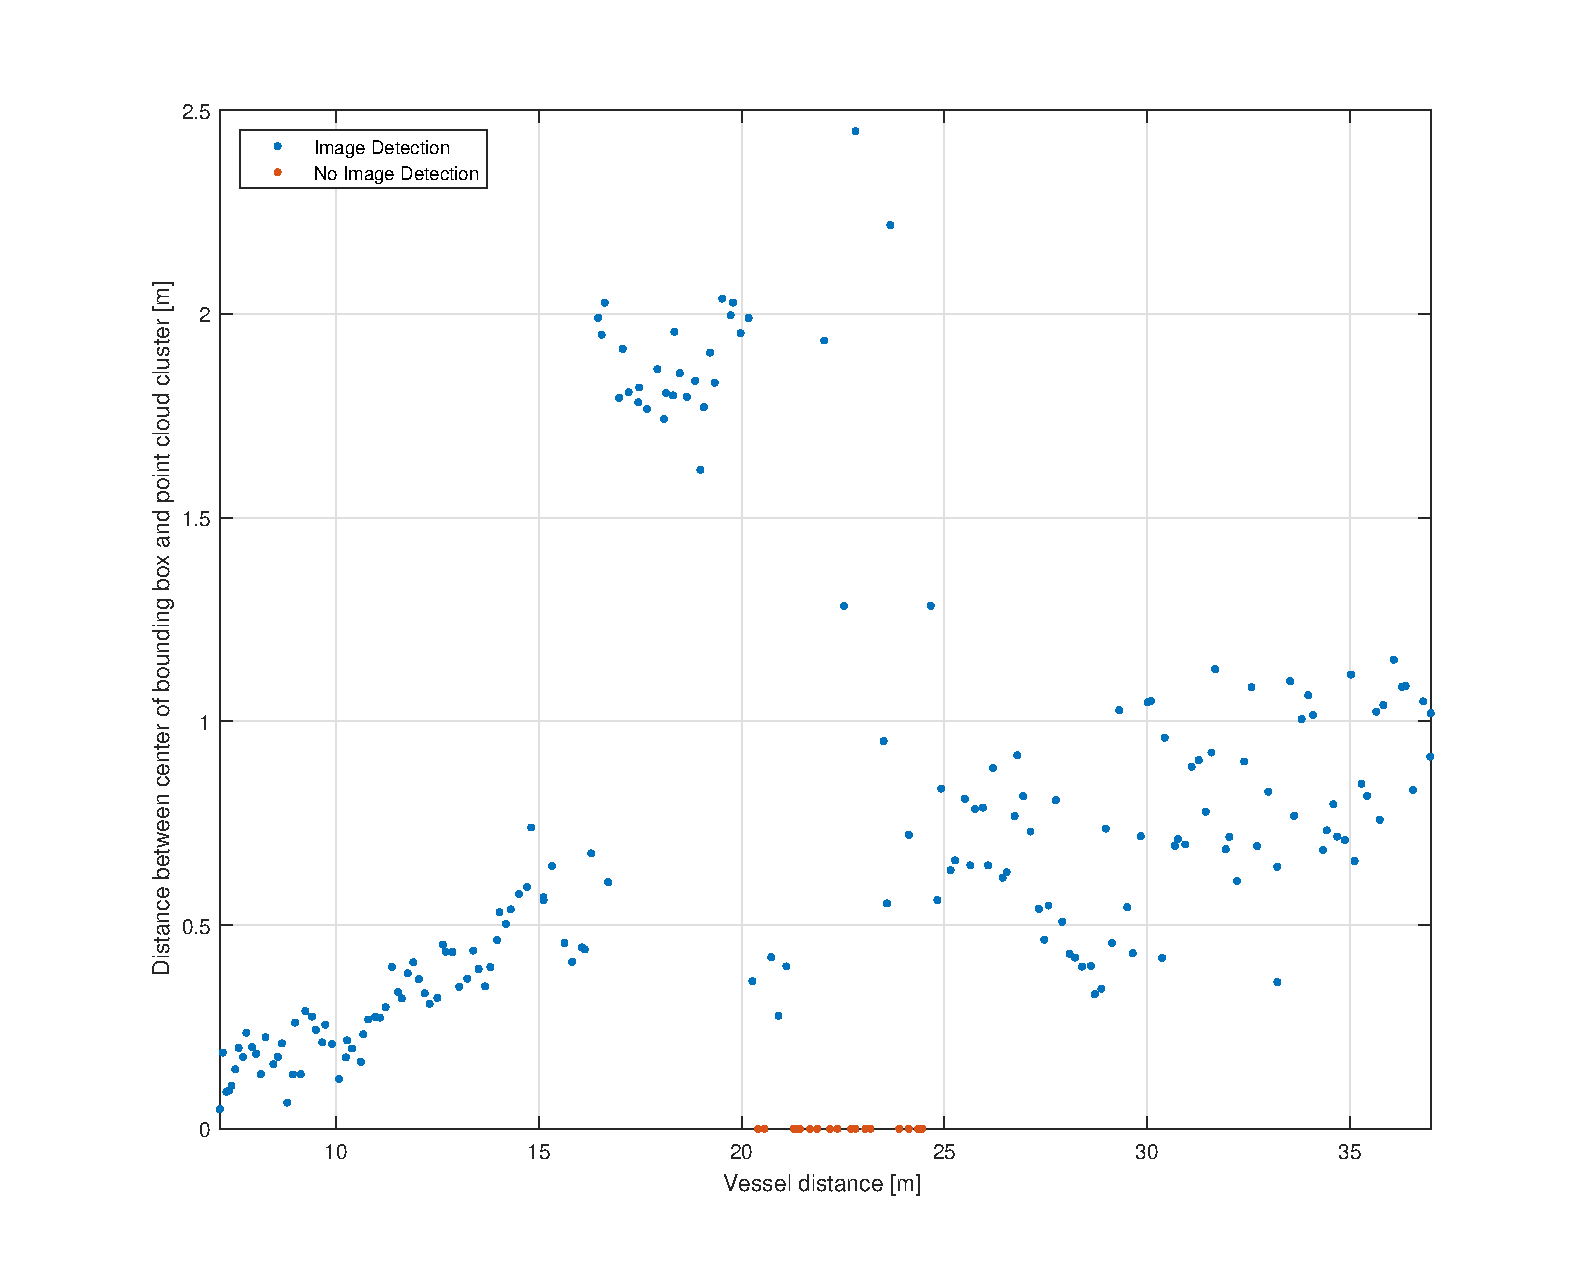
\includegraphics[width=\linewidth]{fig/exp_2_detect_dist.eps}
	\caption{Distance from the center of the bounding\\ box to the point cloud cluster centroid vs.\\ distance to target.}
	\label{fig:sub_ex2_detect_dist}
\end{subfigure}%
\begin{subfigure}[t]{.5\textwidth}
	\centering
	\includegraphics[width=\linewidth]{fig/exp_2_probs.eps}
	\caption{Estimate for probability of detection based on range.}
	\label{fig:sub_ex2_prob}
\end{subfigure}
\caption{Results from experiment 2.}
\label{fig:ex2_plot}
\end{figure}
\begin{figure}[H]
	\centering
	\begin{subfigure}[t]{.5\linewidth}
		\centering
		\includegraphics[width=\linewidth]{fig/exp_2_problem.png}
		\caption{Background ship confusing the\\ detection of the target.}
		\label{fig:sub_ex2_issue}
	\end{subfigure}%
	\begin{subfigure}[t]{.5\linewidth}
		\centering
		\includegraphics[width=\linewidth]{fig/exp2_past_problem.png}
		\caption{Large enough separation to be detected as two separate ships}
		\label{fig:sub_ex2_issue2}
	\end{subfigure}
	\caption{Two examples of multiple ships being detected and classified as one.}
	\label{fig:issues_ex2}
\end{figure} 
\begin{table}[H]
	\centering
	\begin{tabularx}{.7\linewidth}{L c}
		\toprule
		Number of point clouds & 203\\
		\midrule
		Number of detections & 186\\
		\midrule
		Estimated probability of detection in image & 0.9163 \\
		\bottomrule
	\end{tabularx}
	\caption{Data from experiment 1.}
	\label{tab:exp1}
\end{table}
\subsection{Experiment 3}
\subsection{Experiment 4}
\subsection{Experiment 5}
\subsection{Experiment 6}
\subsection{Experiment 7}
\cleardoublepage